We describe the problem statement, the approach, the dataset, and the main experimental results of AppEvolve.

\subsection{Problem Statement}\label{sec:problem}
%Consider two Android API versions: $oldAPIs = [m_1, m_2, ..., m_k]$ and $newAPIs = [m_1', m_2', ..., m_l']$. An API usage may involve one or more methods from either $oldAPIs$ or $newAPIs$. An API usage change from the $oldAPIs$ to the $newAPIs$ can be defined as a change from one or more methods from the $oldAPIs$ to one or more methods from the $newAPIs$, which can be written as $[m_1, m_2, ..., m_p] \rightarrow [m_1', m_2', ..., m_q']$. The goal of automatic update of Android apps is to update usages of $oldAPIs$ to $newAPIs$ based on the API usage change while also maintaining backward compatibility.

AppEvolve targets the case where a set of one or more methods in one
version of the Android API are replaced by another set of one or more
methods in a later version of the Android API.  The goal of AppEvolve is to
automatically update Android apps that use the old methods so that they use
the new methods, while retaining backwards compatability.

%\begin{figure*}[htb]
%	\centering
%	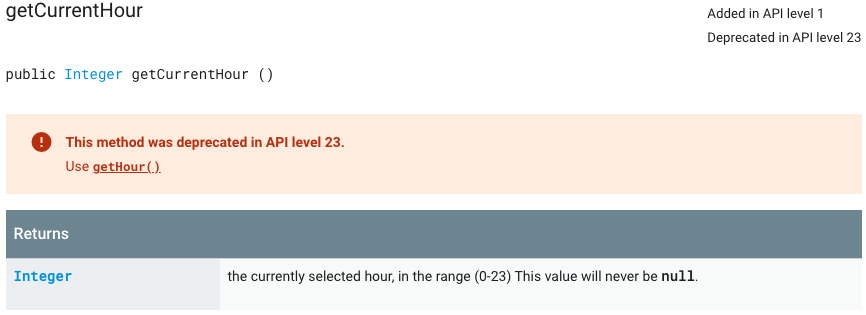
\includegraphics[width=0.8\linewidth]{deprecated-api-example.png}
%	\caption{An example of a deprecated API
%	}
%	\label{fig:deprecated_api_example}
%\end{figure*}

To illustrate the API usage update problem, consider a change in the Android API version 23: the method \texttt{getCurrentHour()}, which returns the currently selected hour, was deprecated in version 23 of the Android API and the method \texttt{getHour()} was suggested as its replacement. 

Figure~\ref{fig:deprecated_api_update_example} shows an example of an API
usage change that modifies a usage of method \texttt{getCurrentHour()} to
its replacement method \texttt{getHour()}. Given this example, one can
learn abstracted relevant edits as shown in
Figure~\ref{fig:deprecated_api_update_edits}. These edits update a
deprecated method usage to a replacement method usage. In these edits,
backward compatibility is achieved by checking the version number of the
mobile OS running the app. If the version is greater than or equal to a
certain version number, the replacement method is used. Otherwise, the
deprecated method is used.

\begin{figure}[htb]
\centering
\begin{lstlisting}[language=diff,numbers=none]
private long addEventToGCal() {
  ...
  int hourInt;
  int minInt;
- hourInt = timepicker.getCurrentHour();
- minInt = timepicker.getCurrentMinute();
+ if (android.os.Build.VERSION.SDK_INT >= 
+       android.os.Build.VERSION_CODES.M) {
+  hourInt = timepicker.getHour();
+  minInt = timepicker.getMinute();
+ } else {
+  hourInt = timepicker.getCurrentHour();
+  minInt = timepicker.getCurrentMinute();
+ }
  ...
}
\end{lstlisting}
\caption{A deprecated API-usage update}
\label{fig:deprecated_api_update_example}
\end{figure}

\begin{figure}[htb]
\centering
\begin{lstlisting}[language=diff,numbers=none]
- $T = $T.getCurrentHour();
+ if (android.os.Build.VERSION.SDK_INT >= 
+       android.os.Build.VERSION_CODES.M) {
+  $T = $T.getHour();
+ } else {
+  $T = $T.getCurrentHour();
+ }
\end{lstlisting}
\caption{Edits for updating deprecated method \texttt{getCurrentHour()}}
\label{fig:deprecated_api_update_edits}
\end{figure}

\subsection{Approach}
\toolname\ takes as input a target app to update and a mapping from a
deprecated API method \jl{Only one?  If so, maybe the first paragraph of
  Section 2A should reflect this.} to its replacement API method(s). The
framework of \toolname\ is shown in Figure~\ref{fig:framework}. The
framework is divided into four phases: {\em API-Usage Analysis}, {\em
  Update Example Search}, {\em Update Example Analysis} and {\em API-Usage
  Update}.

In the {\em API-Usage Analysis} phase, \toolname\ accepts as input an {\em
  API Usage Change} and a {\em Target App}. An {\em API Usage Change}
describes the mapping from a deprecated API method to its corresponding
replacement API method \jl{Now there is only one replacement method as
  well.  This should be consistent.} \jl{Should we say that the usage
  change may come eg from the documentation?}. A {\em Target App} is an app
that contains a usage of the deprecated API method and requires updates to
make use of the replacement API method. Given these two inputs,
\toolname\ pinpoints the location of the deprecated API usage in the {\em
  Target App}. In the {\em Update Example Search} phase,
\toolname\ searches GitHub for examples of API usage updates that modify
the usage of the deprecated API method to include the usage of the
replacement API methods. In the {\em Update Example Analysis} phase,
\toolname\ generates generic patches \jl{The same as an abstracted relevant
  edit?} from the examples of API usage updates and ranks these patches. In
the {\em API Usage Update} phase, \toolname\ tries to apply the ranked
patches one by one and returns the {\em Evolved Target App} if any of the
edits is successful and validated.

\begin{figure*}[t]
	\centering
	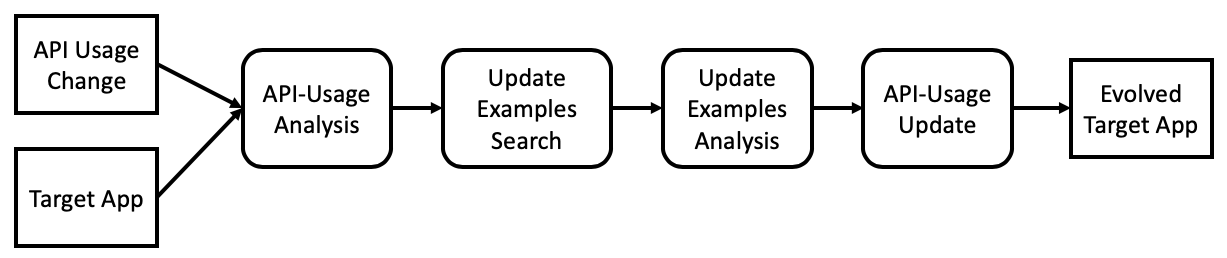
\includegraphics[width=0.8\linewidth]{framework.png}
	\caption{Framework of AppEvolve}
	\label{fig:framework}
\end{figure*}

We next describe each of the above phases in detail.
\subsubsection{API-Usage Analysis}
\toolname\ finds the location where the deprecated API method specified in
the {\em API Usage Change} is used inside the {\em Target App}. Consider
the deprecated API method \texttt{getCurrentHour()} mentioned in
Section~\ref{sec:problem}.  In this case, the {\em API Usage Change} is the replacement of the deprecated method \texttt{getCurrentHour()} with method \texttt{getHour()}. Given this information, \toolname\ finds the location in the {\em Target App} that calls deprecated method \texttt{getCurrentHour()}. %Suppose
                                                                                                                                                                                                                                                                                                                 %that
                                                                                                                                                                                                                                                                                                                 %the
                                                                                                                                                                                                                                                                                                                 %{\em
                                                                                                                                                                                                                                                                                                                 %Target
                                                                                                                                                                                                                                                                                                                 %App}'s
                                                                                                                                                                                                                                                                                                                 %update
                                                                                                                                                                                                                                                                                                                 %location
                                                                                                                                                                                                                                                                                                                 %is
                                                                                                                                                                                                                                                                                                                 %as
                                                                                                                                                                                                                                                                                                                 %shown
                                                                                                                                                                                                                                                                                                                 %in
                                                                                                                                                                                                                                                                                                                 %Figure~\ref{fig:deprecated_api_update_target},
                                                                                                                                                                                                                                                                                                                 %\toolname\ records
                                                                                                                                                                                                                                                                                                                 %this
                                                                                                                                                                                                                                                                                                                 %location
                                                                                                                                                                                                                                                                                                                 %for
                                                                                                                                                                                                                                                                                                                 %applying
                                                                                                                                                                                                                                                                                                                 %the
                                                                                                                                                                                                                                                                                                                 %updates
                                                                                                                                                                                                                                                                                                                 %later
                                                                                                                                                                                                                                                                                                                 %on.

\subsubsection{Update Example Search}
\toolname\ searches for apps in GitHub that use both the deprecated and the replacement API methods in their latest versions.  For each such app, AppEvolve looks through the app history to find the commit where the replacement API methods are added. This is intended to find examples that produce a backward compatible Android app. We need both methods in an example since the Android app might be run in devices with either an older version of the Android OS (in which possibly only the deprecated method exists) or a newer version of the Android OS (in which possibly only the replacement method exists). Given these apps, \toolname\ finds changes that add the replacement API method to the app code that already contains the deprecated API method. These changes are the examples that can be used to update deprecated API method usages in other apps.

\subsubsection{Update Example Analysis}
Given the examples found in GitHub, AppEvolve translates each example to a generic patch. It does so by identifying edits related to the API usage via intraprocedural forward and backward dependency analysis on the variables involved in the API usage. Variables that are used in statement affected by the edits but not defined by the edits themselves are considered as context variables. All variables in the edits are then abstracted. Given the generic patches, AppEvolve computes the the common core of these generic patches. The common core is defined as the longest subsequence of edits that are shared across the patches. The patches are then ranked based on their distance to the core.

\subsubsection{API-Usage Update}
Given a {\em Target App}, AppEvolve applies the generic patches according to their computed rank in the previous phase. When applying a patch, AppEvolve first finds mappings of context variables to variables in the {\em Target App}. For each such mapping, AppEvolve tries to apply the patch. If the edits are successfully applied, AppEvolve returns the {\em Evolved Target App}.

\subsection{Dataset}
For the target apps, the AppEvolve paper used 15 real-world apps from the F-droid repository.\footnote{\url{https://fdroid.org}} These  apps cover 20 API usages in 41 locations. AppEvolve authors selected five apps each for Android API versions 22, 23, and 25. For each API version, the API change is manually identified by reading the API
documentation. Using the API change, the API usage in each app is guaranteed to be: (1) different from the ones in the other apps and (2)
updated in the subsequent API version. 

\subsection{Results}
When applied to the 15 apps considered, AppEvolve was able to update 17 out of 20 API usages (85\% success rate) and 37 out of 41 of their occurrences across the apps.
